\chapter{Principais opções alteradas na configuração do \textit{kernel}}
\label{cap:kernelconfig}

As configurações requeridas pelo Preempt\_RT e pelo RTAI estão marcadas com seus respectivos nomes. 

A opção \textit{Fully Preemptible kernel (RT)} só está disponível após a aplicação do \textit{patch} Preempt\_RT. 

A opção \textit{Interrupt pipeline} só está disponível após a aplicação do \textit{patch} HAL do RTAI. 

O arquivo de configuração utilizado tem como base a versão \textit{vanilla} dos \textit{kernels} utilizados.

\begin{itemize}
    \item Kernel 32 bits
    	\begin{itemize}
    		\item {[} {]} 64-bit kernel
    	\end{itemize}
    \item General setup > Timers subsystem
    	\begin{itemize}
    		\item {[}*{]} High Resolution Timer Support
    		\item {[}*{]} Enable Loadable module support (RTAI)
    		\item {[} {]} Module versioning support (RTAI)
    	\end{itemize}
    \item Processor type and features
    	\begin{itemize}
    		\item {[} {]} Symmetric multi-processing support
    		\item Processor family > (X) Pentium-Classic
    		\item Preemption Model > (X) Fully Preemptible kernel (RT) (Preempt\_RT)
    		\item {[}*{]} Interrupt pipeline (RTAI)
    		\item Time frequency > (X) 1000HZ
    		\item {[} {]} AMD MCE features (RTAI)
    	\end{itemize}
    \item Power Management and ACPI options
    	\begin{itemize}
    		\item {[} {]} ACPI (Advanced Configuration and Power Interface) Support
    		\item CPU Frequency scaling > {[} {]} CPU Frequency scaling
    		\item CPU Idle > {[} {]} CPU Idle PM support
    	\end{itemize}
    \item File systems > Pseudo filesystems
    	\begin{itemize}
    		\item {[}*{]} /proc file system support (RTAI)
    	\end{itemize}
    \item Kernel hacking
    	\begin{itemize}
    		\item {[} {]} Debug preemptible kernel
    		\item {[} {]} Debug the x86 FPU code
    	\end{itemize}
\end{itemize}

\chapter{Fluxograma dos programas de teste}
\label{cap:fluxograma}
\begin{figure}[!htb]
    \centering
    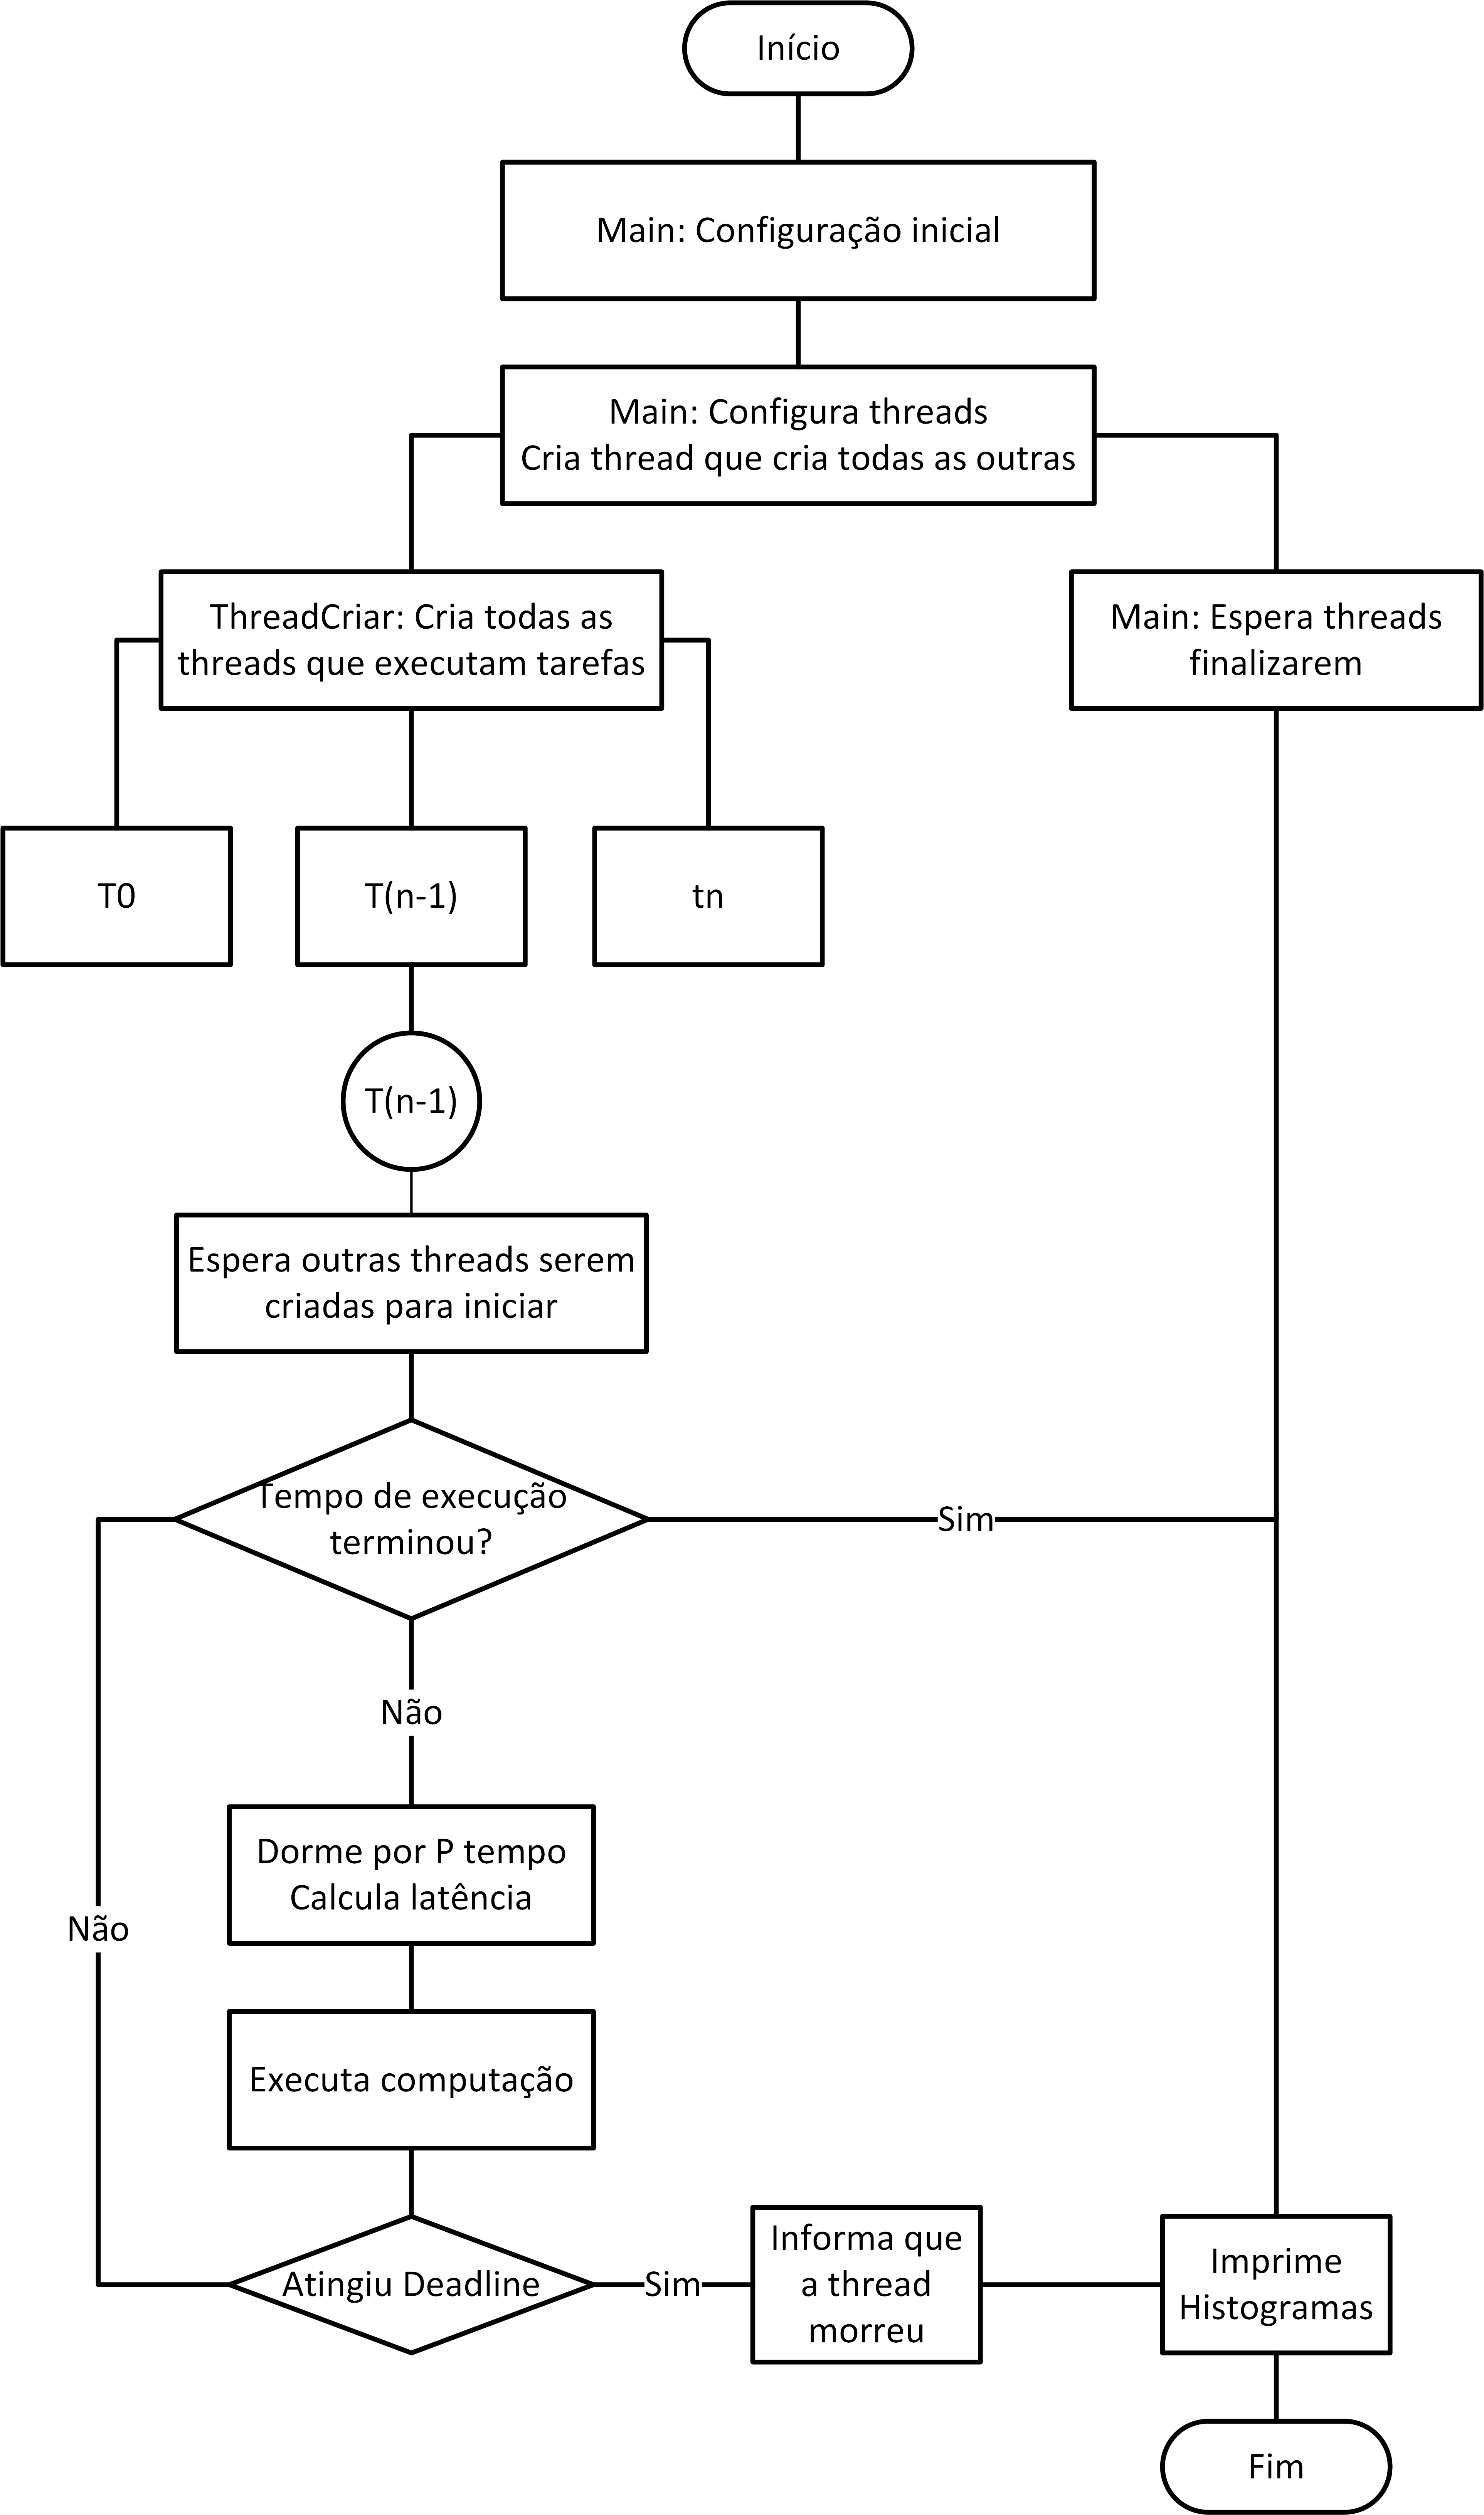
\includegraphics[scale=0.80]{FluxoProgramaDeTestes}
    \label{fluxograma}
\end{figure}

\chapter{\textit{Script} para inicialização do RTAI (rtai-init.bash)}
\label{cap:script}
\lstset{literate=
  {á}{{\'a}}1 {é}{{\'e}}1 {í}{{\'i}}1 {ó}{{\'o}}1 {ú}{{\'u}}1
  {Á}{{\'A}}1 {É}{{\'E}}1 {Í}{{\'I}}1 {Ó}{{\'O}}1 {Ú}{{\'U}}1
  {â}{{\^a}}1 {ê}{{\^e}}1 {î}{{\^i}}1 {ô}{{\^o}}1 {û}{{\^u}}1
  {Â}{{\^A}}1 {Ê}{{\^E}}1 {Î}{{\^I}}1 {Ô}{{\^O}}1 {Û}{{\^U}}1
  {ű}{{\H{u}}}1 {ő}{{\H{o}}}1 {ã}{{\H{a}}}1
  {ç}{{\c c}}1 {Ç}{{\c C}}1 {«}{{\guillemotleft}}1 {»}{{\guillemotright}}1
}
\lstset{language=bash}
\begin{lstlisting}[frame=single]
#!/bin/bash

# Carregando os módulos do RTAI
sudo insmod /usr/realtime/modules/rtai_hal.ko
sudo insmod /usr/realtime/modules/rtai_sched.ko
sudo insmod /usr/realtime/modules/rtai_fifos.ko
sudo insmod /usr/realtime/modules/rtai_sem.ko
sudo insmod /usr/realtime/modules/rtai_mbx.ko
sudo insmod /usr/realtime/modules/rtai_msg.ko
sudo insmod /usr/realtime/modules/rtai_shm.ko
sudo insmod /usr/realtime/modules/rtai_smi.ko
sudo insmod /usr/realtime/modules/latency_rt.ko

# Criando as variáveis para compilação
export CFLAGS=$(/usr/realtime/bin/./rtai-config --lxrt-cflags)
export LDFLAGS=$(/usr/realtime/bin/./rtai-config --lxrt-ldflags)
\end{lstlisting}

Para que as variáveis criadas pelo \textit{script} possam ser utilizadas por todos os usuários é preciso utilizar a notação ponto seguido por espaço:

\begin{lstlisting}[frame=single]
$ . rtai-init
\end{lstlisting}